%% ============================================================
%%  Anchoring Options to an Incomplete Forward Curve
%%  Elsevier preprint (elsarticle, single-column review format)
%% ============================================================
\documentclass[preprint,12pt,authoryear]{elsarticle}

% ---------- packages ----------
\usepackage[T1]{fontenc}
\usepackage[utf8]{inputenc}
\usepackage{amsmath,amssymb,amsthm}
\usepackage{mathtools}
\usepackage{graphicx}
\usepackage{booktabs}
\usepackage{multirow}
\usepackage[hidelinks]{hyperref}
\usepackage{xcolor}
\usepackage{caption}
\captionsetup{font=small,labelfont=bf}

% ---------- spacing / float control (keeps figures tight) ----------
\setlength{\textfloatsep}{14pt plus 2pt minus 2pt}
\setlength{\floatsep}{12pt plus 2pt minus 2pt}
\setlength{\intextsep}{12pt plus 2pt minus 2pt}
\renewcommand{\topfraction}{0.85}
\renewcommand{\bottomfraction}{0.70}
\renewcommand{\textfraction}{0.10}
\renewcommand{\floatpagefraction}{0.75}

% ---------- theorem environments ----------
\newtheorem{proposition}{Proposition}
\newtheorem{assumption}{Assumption}
\newtheorem{remark}{Remark}

% ---------- notation shorthands ----------
\newcommand{\Q}{\mathbb{Q}}
\newcommand{\PP}{\mathbb{P}}
\newcommand{\E}{\mathbb{E}}
\newcommand{\TRY}{\ensuremath{\mathrm{TRY/MWh}}}
\newcommand{\dif}{\mathrm{d}}

\journal{Working paper}

\begin{document}

\begin{frontmatter}

\title{Anchoring Options to an Incomplete Forward Curve:\\
Identification and Out-of-Sample Evidence from\\
Turkish Electricity}

\author[ozu]{Onat Uzkan}
\ead{onat.uzkan@ozu.edu.tr}
\author[itu]{Koray Ömercan Saçlı}
\ead{sacli24@itu.edu.tr}

\address[ozu]{Department of Mechanical Engineering, Özyeğin University,
Istanbul, Türkiye}
\address[itu]{Department of Mechanical Engineering, Istanbul Technical
University, Istanbul, Türkiye}

\begin{abstract}
Electricity options in emerging markets must be valued without the two
ingredients that standard derivative pricing takes for granted: a traded
option surface from which risk-neutral parameters could be read off, and a
continuous forward curve. The Turkish market offers only a sparse strip of
monthly baseload forward quotes, and even that strip leaves the nearest
delivery month unquoted. This paper develops a valuation framework that
separates what such a market identifies from what it does not. An hourly curve
is constructed as the smoothest one consistent with the observed monthly
averages, imposed as hard equality constraints, and a two-regime
Ornstein--Uhlenbeck residual with residual-demand-driven time-varying transition
probabilities is attached in a centred form, so that $\E^{\Q}[P_t]=F(t)$ holds
for every admissible parameter vector. The construction isolates the forward
level as the only market-identified object, leaving volatility and regime risk
premia as explicit, separately reported assumptions rather than implicit
consequences of a fitting procedure. Expiry-hour European options are priced on
this structure through a coupled moment-ODE and finite-difference system,
cross-validated against Monte Carlo simulation, with the full sensitivity of the
resulting prices to each unidentified input reported. The framework is then evaluated against realised prices. Over the first half of
2026 an exceptional hydrological year drove Turkish spot prices far below the
December 2025 forward strip, producing a mean bias of $-1{,}019$ \TRY{} across
5{,}088 delivery hours. Replaying the curve construction at seven valuation
dates between 2022 and 2025 shows that this outcome was not exceptional: the
pooled bias over 49 date-month observations averages $-603$ \TRY{} ($-18\%$),
realised prices fell below the strip at five of seven dates and rose above it at
two, and the 2026 result lies inside the interquartile range of the date means.
Since the model reproduces the strip exactly, this error is inherited from the
forward market rather than generated by the pricing layer. The monthly strip is
therefore a biased and sign-unstable predictor of realised baseload prices, and
that, rather than any property of the pricing scheme, bounds what
forward-anchored valuation can deliver in this market.
\end{abstract}

\begin{keyword}
electricity option valuation \sep regime switching \sep time-varying transition
probabilities \sep hourly forward curve \sep Turkish electricity market \sep
incomplete markets
\end{keyword}

\end{frontmatter}

\section{Introduction}
\label{sec:intro}

Valuing an electricity option requires a probability measure under which the
expected discounted payoff is the price. Where a liquid option surface exists,
that measure is recovered from traded instruments: implied volatilities pin down
the diffusion and the forward curve pins down the drift. Neither ingredient is
available in most emerging electricity markets. The Turkish market is a
representative case. Its organised derivative segment, the \emph{Vadeli Elektrik
Piyasası} (VEP) operated by EPİAŞ, lists monthly baseload futures, and
exchange-traded options on power are effectively absent. A practitioner who needs
the value of a call on the hourly spot price at a specific delivery hour
therefore faces two gaps at once: the forward curve is observed only as a coarse
strip of monthly averages, and the risk-neutral distribution around that curve is
not observed at all.

Each gap has been addressed separately in a mature literature. On the
distributional side, regime switching in power prices is well established.
Building on \citet{Hamilton1989}, \citet{Huisman2003} and \citet{Deng2000} argue
that spike behaviour is better represented by a switch between a calm
mean-reverting state and a distinct spike state than by adding jumps to a single
process. \citet{JanczuraWeron2010} compare specifications systematically and find
that independent-spike-regime models with heavy tails dominate simpler
alternatives, consistent with the tail evidence in \citet{Weron2009};
\citet{Deschatre2021} survey the resulting model class. Allowing the switching
probabilities to respond to fundamentals, following \citet{Diebold1994} and
\citet{Filardo1994}, tightens the fit further: \citet{Mount2006} and
\citet{KanamuraOhashi2008} make transition probabilities depend on load and
reserve margin, and \citet{KarakatsaniBunn2008} show that intra-day regime
dynamics carry economic content rather than statistical artefact. Residual
demand, load net of non-dispatchable renewable generation, is the natural
covariate. \citet{Wagner2014} and \citet{Do2021} document its role in price
formation, and the merit-order literature
\citep{Sensfuss2008,Ketterer2014,Clo2015} explains the mechanism: renewable
output displaces the marginal thermal unit and shifts the supply stack. For
Türkiye, \citet{SirinYilmaz2020} quantify the merit-order effect through quantile
regression, while \citet{Ugurlu2018} and \citet{Ertugrul2022} document the
forecasting properties of Turkish spot prices.

On the curve-construction side, turning coarse forward quotes into a granular
curve is equally well studied. \citet{LuciaSchwartz2002} establish the
decomposition of a power price into a deterministic component and a
mean-reverting stochastic residual that underlies most subsequent work;
\citet{FletenLemming2003} pose curve construction as a smoothing problem
constrained to reproduce observed contract prices; \citet{Borak2008} model
forward curve dynamics semi-parametrically; \citet{Kiesel2019} and
\citet{Caldana2017} construct hourly curves for European markets. The common
structure is a smoothness objective subject to arbitrage-free reproduction of the
observed strip.

Pricing on a regime-switching state space is likewise a solved numerical problem.
\citet{BuffingtonElliott2002} and \citet{JobertRogers2006} give the
Markov-modulated framework, \citet{BoyleDraviam2007} and \citet{Huang2011}
develop finite-difference schemes for the coupled systems,
\citet{ChenForsyth2010} apply them to gas storage, and \citet{Zeng2017} compare
finite-difference and Monte Carlo approaches directly. The closest antecedent to
the present study is \citet{Paraschiv2015}, who combine spot and forward
information within a regime-shifting specification. Our departure is to treat the
boundary between the two as an identification question rather than an estimation
one.

That question is what remains open. When a market supplies a forward strip and
nothing else, which parameters of such a model are determined by data, and which
are assumptions the analyst has imported? The distinction is easily obscured. A
model calibrated to reproduce a forward strip to numerical precision looks
calibrated. Where switching parameters and volatilities have been estimated on a
historical sample under the physical measure $\PP$ and are then used for pricing
under $\Q$ without adjustment, the resulting value embeds an untested assumption
that the market charges no premium for regime or volatility risk.
\citet{Janczura2014} constructs such premia explicitly within a regime-switching
framework, \citet{BessembinderLemmon2002} derive equilibrium forward premia from
hedging pressure, and \citet{LongstaffWang2004} and \citet{Algieri2021} measure
them empirically. The premium is a real economic object; it does not vanish
because it was not estimated.

\paragraph{Contribution.}
The separation is made explicit here, and a valuation framework is built around
it. Four contributions follow.

First, a \emph{forward-centred} representation is proposed, in which the spot
price is written as $P_t = F(t) + X_t - \E^{\Q}[X_t]$, with $F$ the
equality-constrained hourly curve and $X$ a two-regime Ornstein--Uhlenbeck
residual with time-varying transition probabilities. Subtracting the residual's
own mean is not a normalisation of convenience: it renders $\E^{\Q}[P_t]=F(t)$ an
algebraic identity holding for every admissible parameter vector, so that the
market-identified first moment is structurally insulated from the unidentified
higher moments. This is established in Proposition~\ref{prop:centering} and
verified numerically across the parameter space explored below, including under
measure changes.

Second, the unidentified inputs are made auditable rather than invisible. Every
parameter carries a provenance label distinguishing calibrated quantities from
inherited historical estimates, derived reconstructions and outright assumptions
(Table~\ref{tab:provenance}), and each is subjected to a controlled sensitivity
experiment in which it alone varies. The risk-neutral drift channel is
implemented as an explicit, switchable perturbation whose default value of zero
reproduces the physical-measure baseline exactly, which makes the zero-premium
assumption a visible choice rather than a silent default.

Third, the framework's principal weakness is shown to lie outside its pricing
layer. Using $5{,}088$ hours of spot prices realised after the valuation date, we
find that the December 2025 forward strip missed the subsequent outcome by a mean
of $-1{,}019$ \TRY, with monthly signed errors from $-24\%$ to $-76\%$, during a
period of exceptionally strong hydrological conditions and record renewable
output. Replaying the curve construction at seven valuation dates from 2022
onward places that outcome in context: it is large but not exceptional, and the
strip's error is negative on average yet unstable in sign. To our knowledge the
predictive performance of the Turkish monthly forward strip has not previously
been measured over a multi-year sample, and the resulting distribution bounds
what forward-anchored valuation can deliver here.

Fourth, a methodological failure and its correction are documented in full. An
initial specification inherited its mean-reversion speed from an autoregressive
fit to the untransformed price level, producing a within-regime half-life of
roughly nineteen years and residual dispersion seven to thirteen times wider than
the realised sample exhibits. Diagnosis required separating within-regime
persistence from the marginal persistence of the switching process, quantities
that differ here by four orders of magnitude. A framework whose sensitivity to a
single inherited coefficient exceeds a factor of four is one whose provenance
discipline is not optional, and the episode is reported on that basis.

Section~\ref{sec:market} describes the market, contract and data;
Section~\ref{sec:curve} develops the hourly curve; Section~\ref{sec:residual}
specifies the residual dynamics and the centring identity;
Section~\ref{sec:valuation} derives the moment system and pricing equation;
Section~\ref{sec:provenance} sets out parameter provenance; and
Section~\ref{sec:results} reports calibration quality, the option surface, the
sensitivity battery and the realised evaluation.

\section{Market, contract and data}
\label{sec:market}

\subsection{The Turkish wholesale electricity market}

Wholesale electricity in Türkiye clears through EPİAŞ, the market operator. The
day-ahead market produces an hourly clearing price, the \emph{Piyasa Takas
Fiyatı} (PTF), for every delivery hour of the following day \citep{EPIAS2025}.
PTF is the reference price for physical settlement and the underlying taken here
for option valuation. Prices are quoted in Turkish lira per megawatt-hour and are
subject to administratively set ceiling and floor levels revised periodically
\citep{EPDK2024}.

The organised forward segment, VEP, lists monthly baseload futures. A contract
for delivery month $m$, denoted \texttt{EBM}$mm$\texttt{yy}, settles against the
arithmetic mean of PTF over every delivery hour of that month. This averaging
structure is the first source of the identification problem addressed here. A
monthly baseload quote constrains the \emph{average} of $720$ to $744$ hourly
forward prices and says nothing about how that average is distributed across
hours. Two curves with identical monthly means but different intraday shapes are
equally consistent with the same quote, yet imply materially different values for
an option written on a single delivery hour.

Two features make the market a useful laboratory for these questions. Renewable
penetration has grown quickly, so residual demand fluctuates over a wide range
and the merit-order mechanism transmitting it into price is strong
\citep{SirinYilmaz2020}. And the lira has depreciated substantially over the
period from which historical parameters must be drawn, so nominal price series
mix genuine dynamics with monetary trend. Consequences of the second feature are
taken up in Section~\ref{sec:limitations}.

\subsection{The contract}

The instrument valued here is a European call on the PTF observed at a single
expiry hour $T$,
\begin{equation}
  V_0 \;=\; e^{-rT}\,\E^{\Q}\!\left[(P_T-K)^+\right],
  \label{eq:payoff}
\end{equation}
where $P_T$ is the hourly clearing price at $T$, $K$ the strike and $r$ a flat
continuously compounded annual rate. This is not the monthly baseload contract
that VEP quotes. The distinction is enforced in the implementation: monthly
quotes are represented by an object that raises an error if accessed as a point
forward, since conflating the two is the shortcut the data structure most invites.

\subsection{Valuation date and samples}

The valuation timestamp is 2025-12-31 20:00 UTC, the final hour of the historical
sample, at which the observed spot is $2{,}917.78$ \TRY. Six monthly baseload
quotes were observed at that date, for delivery months February through July 2026
(Table~\ref{tab:quotes}). January 2026 carries no quote. This is not an avoidable
data gap: the nearest delivery month is the one whose option values matter most
for short-dated contracts, and it is precisely the month the strip does not
price. Section~\ref{sec:anchor} treats it explicitly.

Two further samples enter. The regime covariate is a standardised residual demand
series $z_t$ at hourly frequency, standardised using the training scaler of the
underlying estimation exercise ($N=61{,}361$). The realised evaluation uses hourly
PTF for January through July 2026, $5{,}088$ hours, retrieved from the EPİAŞ
transparency platform after the fact. The evaluation sample is strictly posterior
to the valuation timestamp; no observation from it enters calibration, parameter
estimation or model selection. This is verified structurally rather than by
assertion, through a guard test that fails if any fitting routine is exposed to a
timestamp at or beyond the valuation cutoff.

\begin{table}[htbp]
\centering
\caption{Observed VEP monthly baseload quotes at the valuation date
(2025-12-31), in \TRY.}
\label{tab:quotes}
\small
\begin{tabular}{@{}llrr@{}}
\toprule
Contract & Delivery month & Delivery hours & Quote \\
\midrule
EBM0226 & February 2026 & 672 & 2{,}900.99 \\
EBM0326 & March 2026    & 744 & 2{,}556.31 \\
EBM0426 & April 2026    & 720 & 2{,}500.66 \\
EBM0526 & May 2026      & 744 & 2{,}506.25 \\
EBM0626 & June 2026     & 720 & 2{,}245.33 \\
EBM0726 & July 2026     & 744 & 3{,}558.19 \\
\midrule
\multicolumn{2}{@{}l}{January 2026} & 744 & \emph{unquoted} \\
\bottomrule
\end{tabular}
\end{table}

The strip carries information worth noting before any modelling. The market
priced a pronounced decline from February to June followed by a sharp July
rebound of roughly $58\%$ over the June level, a shape consistent with
cooling-driven summer peaks and high spring hydro and solar availability. The
hourly curve must therefore accommodate a large discontinuity at the June--July
boundary originating in the data rather than in the interpolation method, a point
verified in Section~\ref{sec:curvefit}.

\section{The hourly forward curve}
\label{sec:curve}

Figure~\ref{fig:pipeline} summarises how the components of the framework fit
together and, more importantly, where market information enters and where it
does not. The upper path carries observed prices into the forward curve. The
lower path carries historical estimates into the residual dynamics. The two
meet only at the centring step, and the separation is what makes the
identification argument of this paper possible.

\begin{figure}[htbp]
\centering
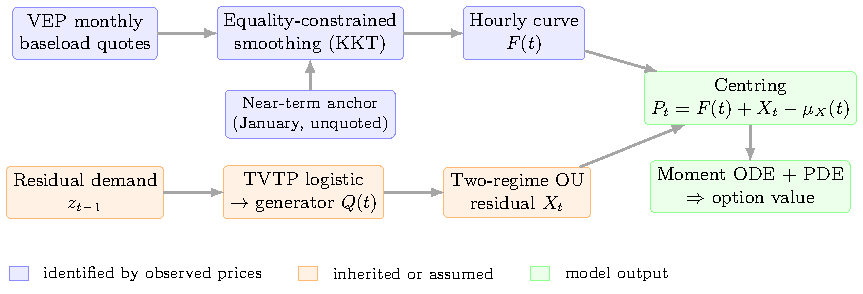
\includegraphics[width=0.92\textwidth]{figures/pipeline.pdf}
\caption{Structure of the valuation framework. Blue elements are identified by
observed prices; orange elements are inherited from historical estimation or
assumed. Only the first moment of the price distribution is determined by the
market path; volatility and regime risk premia are not. (Vector source:
\texttt{figures/pipeline\_src.tex}.)}
\label{fig:pipeline}
\end{figure}

\subsection{The averaging constraint}

Let $\mathcal{H}_m$ denote the set of delivery hours of month $m$ and
$\mathrm{VEP}_m$ the observed baseload quote. Settlement against the arithmetic
mean imposes
\begin{equation}
  \frac{1}{|\mathcal{H}_m|}\sum_{h\in\mathcal{H}_m} F(h) \;=\; \mathrm{VEP}_m,
  \qquad m \in \mathcal{M},
  \label{eq:monthly}
\end{equation}
where $\mathcal{M}$ is the set of quoted months. With $N$ hourly unknowns and
$|\mathcal{M}|=6$ constraints, the system is massively underdetermined: in our
configuration $N=5{,}089$ and the constraints fix six linear functionals. The
remaining $N-6$ degrees of freedom are chosen, not identified. We select them by
a smoothness criterion, and we regard that selection as an assumption on the
same footing as any other, not as an estimation result.

\subsection{Roughness-penalised construction}

Write $\mathbf{F}\in\mathbb{R}^{N}$ for the vector of hourly forward prices and
$D_2\in\mathbb{R}^{(N-2)\times N}$ for the second-difference operator,
$(D_2\mathbf{F})_i = F_{i+2}-2F_{i+1}+F_i$. Let $\mathbf{B}$ be a piecewise
baseline that is constant at $\mathrm{VEP}_m$ within each quoted month and
follows the near-term anchor rule of Section~\ref{sec:anchor} elsewhere. The
curve solves
\begin{equation}
  \min_{\mathbf{F}} \;
    w_R\,\lVert D_2\mathbf{F}\rVert_2^{2}
    \;+\; w_A\,\lVert \mathbf{F}-\mathbf{B}\rVert_2^{2}
  \quad\text{subject to}\quad
  A\mathbf{F}=\mathbf{b},
  \label{eq:qp}
\end{equation}
where each row of $A$ implements one instance of \eqref{eq:monthly}, together
with the anchor row. This is a convex quadratic program with linear equality
constraints, and we solve it as a single sparse Karush--Kuhn--Tucker system,
\begin{equation}
  \begin{bmatrix}
    2\left(w_R D_2^{\top}D_2 + w_A I\right) & A^{\top}\\
    A & 0
  \end{bmatrix}
  \begin{bmatrix}\mathbf{F}\\ \boldsymbol{\lambda}\end{bmatrix}
  =
  \begin{bmatrix}2w_A\mathbf{B}\\ \mathbf{b}\end{bmatrix}.
  \label{eq:kkt}
\end{equation}

Because the quotes enter as equality constraints rather than as penalty terms,
the weights $w_R$ and $w_A$ govern only the shape of the curve within months.
They cannot trade off fit against smoothness, and no choice of weights can
violate \eqref{eq:monthly}. This has a consequence for how the resulting fit
should be read, and we state it plainly because the opposite reading is the
natural one: the monthly reproduction error we report in
Section~\ref{sec:curvefit} is of order $10^{-12}$ \TRY, and that number is a
property of the solver, not evidence about the model. A formulation that
reproduces its inputs by construction has not been tested by reproducing them.

\subsection{The unquoted near-term window}
\label{sec:anchor}

January 2026 has no quote, and every option maturity examined here falls inside
it. This is not a gap peculiar to one date. Across the seven valuation dates
used in Section~\ref{sec:multidate}, spanning December 2022 to December 2025,
the nearest delivery month is unquoted at every one: the front contract is
delisted before the month it delivers into begins, so a participant valuing a
short-dated instrument never observes a forward price for the period that
instrument covers. The level over that window must therefore come from an
assumption, and the assumption is a permanent feature of valuation in this
market rather than an occasional inconvenience. Three rules are considered, all
respecting the observed spot at the valuation hour where applicable:

\begin{enumerate}
\item \textbf{\texttt{spot\_flat}}: hold the observed spot $2{,}917.78$ \TRY{}
      flat across the window;
\item \textbf{\texttt{spot\_to\_next\_linear}}: interpolate linearly from the
      observed spot at $t_0$ to the February quote at the month boundary;
\item \textbf{\texttt{flat\_next\_month}}: hold the February quote flat
      backwards across January.
\end{enumerate}

We adopt \texttt{spot\_to\_next\_linear} as the production rule on three
grounds. It satisfies $F(t_0)=P_{t_0}$, so the curve is consistent with the one
spot observation that is not in dispute. It joins the February quote without a
discontinuity at the month boundary, with a residual jump of $0.05$ \TRY{}
against $12$--$47$ \TRY{} at boundaries elsewhere in the curve. And it produces
a non-degenerate term structure across the window, whereas
\texttt{flat\_next\_month} violates $\E[P_{t_0}]=P_{t_0}$ by $17$ \TRY{} and
\texttt{spot\_flat} embeds an unmotivated claim that January is a high-price
month relative to February. Section~\ref{sec:anchorsens} quantifies how much
this choice moves option values, which is the question that matters more than
the choice itself.

\begin{remark}
The near-term anchor is the weakest link in the market path of
Figure~\ref{fig:pipeline}, and its weakness is structural rather than
remediable within the data. Where no quote exists for the delivery period, no
construction can identify its forward level; it can only be assumed, and the
assumption should be reported as a sensitivity range rather than a point.
\end{remark}

\section{Residual dynamics and the centring identity}
\label{sec:residual}

\subsection{Transform and regime structure}

Electricity prices are bounded below by an administrative floor, occasionally
negative in other markets \citep{AustHorsch2020}, and heavy-tailed above. The
underlying estimation exercise works on the inverse hyperbolic sine transform,
\begin{equation}
  y_t = \operatorname{asinh}\!\left(\frac{P_t}{s_P}\right),
  \qquad
  P_t = s_P \sinh(y_t),
  \label{eq:asinh}
\end{equation}
with scale $s_P = 282.48$ \TRY. The transform is odd, defined on the whole real
line and asymptotically logarithmic, so it compresses spikes without the
domain restriction of a log transform.

Let $S_t\in\{0,1\}$ be a continuous-time Markov chain, with state $0$ the calm
regime and state $1$ the stress regime, distinguished by their diffusion
coefficients $\sigma^y_0 \ll \sigma^y_1$. Regime volatilities are inherited
from the underlying estimation as $\sigma^y_0 = 0.003535$ and
$\sigma^y_1 = 0.092407$ per $\sqrt{\text{hour}}$, a ratio of roughly $26$.

\subsection{Time-varying transition probabilities}

Transition probabilities depend on standardised residual demand at a one-hour
lag through a logistic link,
\begin{equation}
  p_{01}(t) = \Lambda\!\left(\alpha_{01}+\gamma_{01} z_{t-1}\right),
  \qquad
  p_{10}(t) = \Lambda\!\left(\alpha_{10}+\gamma_{10} z_{t-1}\right),
  \qquad
  \Lambda(x)=\frac{1}{1+e^{-x}},
  \label{eq:tvtp}
\end{equation}
following \citet{Diebold1994} and \citet{Filardo1994}; consistency of maximum
likelihood estimation for this class with covariate-dependent transitions is
established by \citet{Pouzo2022}, and \citet{Bazzi2017} develop the
score-driven alternative. The lag structure matters for interpretation:
$z_{t-1}$ is the residual demand observed \emph{before} the transition it
governs, so the specification is predictive rather than contemporaneous.

Figure~\ref{fig:tvtp} shows the two fitted transition functions against the
sample distribution of the covariate. Over the bulk of the sample the calm-to-stress
probability exceeds the reverse, and the two cross near $z\approx 1.4$; the
economic reading of that crossing is deferred to Section~\ref{sec:sensitivity},
where the covariate channel is quantified.

\begin{figure}[htbp]
\centering
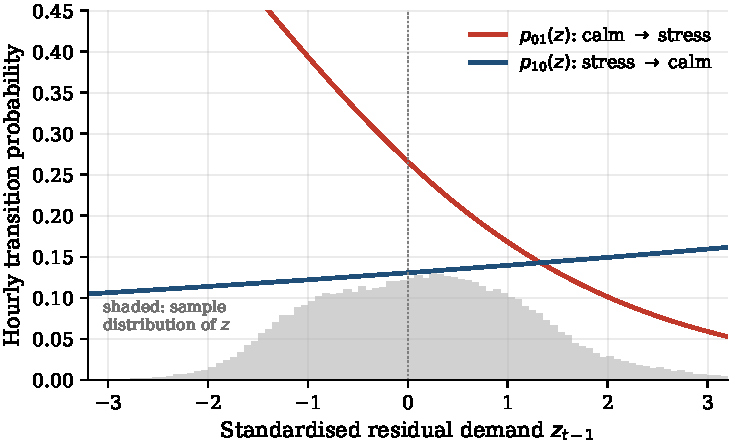
\includegraphics[width=\textwidth]{figures/tvtp_mechanism.pdf}
\caption{Fitted hourly transition probabilities against standardised residual
demand, with the sample distribution of the covariate shaded.}
\label{fig:tvtp}
\end{figure}

The discrete one-step probabilities \eqref{eq:tvtp} are converted to
continuous-time intensities by matrix logarithm. For the two-state chain with
one-step matrix
$\Pi(t) = \begin{psmallmatrix} 1-p_{01} & p_{01}\\ p_{10} & 1-p_{10}\end{psmallmatrix}$
and $s = p_{01}+p_{10}$, the generator is
\begin{equation}
  Q(t) =
  \begin{bmatrix} -q_{01}(t) & q_{01}(t)\\ q_{10}(t) & -q_{10}(t)\end{bmatrix},
  \qquad
  q_{0 1}(t) = \frac{\lambda(t)\,p_{01}(t)}{s(t)},
  \quad
  \lambda(t) = -\ln\!\left(1-s(t)\right),
  \label{eq:generator}
\end{equation}
with $q_{10}$ defined symmetrically, reducing to $q_{ij}\approx p_{ij}/\Delta t$
when $s$ is small. The embedding is exact whenever $s<1$, which holds
throughout our sample. Appendix~\ref{app:transitions} documents the regime
label reconciliation this conversion required.

\subsection{Residual process and price-space diffusion}

Conditional on the regime, the residual follows an Ornstein--Uhlenbeck process
in price space,
\begin{equation}
  \dif X_t = \kappa\left(m_{S_t} - X_t\right)\dif t
             + \sigma^X_{S_t}(t)\,\dif W_t,
  \label{eq:ou}
\end{equation}
with a common mean-reversion rate $\kappa$ and regime-dependent targets $m_i$.
The diffusion coefficient is mapped from transform space to price space by the
delta method applied to \eqref{eq:asinh}. Since
$\dif P/\dif y = \sqrt{P^2+s_P^2}$, evaluating at the forward level gives
\begin{equation}
  \sigma^X_i(t) = \sigma^y_i\,\sqrt{F(t)^2 + s_P^2}\,,
  \label{eq:sigmamap}
\end{equation}
which is state-dependent through $F$ and therefore time-varying even for fixed
$\sigma^y_i$. At $F\approx 2{,}900$ \TRY{} the factor is approximately
$2{,}914$, so the stress-regime price-space diffusion is on the order of
$269$ \TRY{} per $\sqrt{\text{hour}}$.

Two properties of \eqref{eq:ou} deserve emphasis. It is additive rather than
multiplicative, so the model can in principle generate negative terminal
prices; we report the simulated probability of that event in
Section~\ref{sec:results} and treat it as a diagnostic of specification
adequacy. And $\kappa$ is shared across regimes, so regime switching enters the
second moment but not the speed of mean reversion, which keeps the moment
system linear.

\subsection{Forward centring}

The spot price is defined as
\begin{equation}
  \boxed{\;P_t \;=\; F(t) \;+\; X_t \;-\; \mu_X(t),
  \qquad \mu_X(t) \;=\; \E^{\Q}\!\left[X_t\right].\;}
  \label{eq:centering}
\end{equation}

\begin{proposition}[Exact first-moment anchoring]
\label{prop:centering}
Let $X$ satisfy \eqref{eq:ou} with regime process generated by \eqref{eq:generator},
let $\mu_X(t)=\E^{\Q}[X_t]$ be computed under the same measure and the same
parameters used in \eqref{eq:centering}, and let $P$ be defined by
\eqref{eq:centering}. Then
\begin{equation*}
\begin{gathered}
  \E^{\Q}\!\left[P_t\right] = F(t)
  \quad\text{for all } t, \text{ and for every admissible}\\[2pt]
  \left(\kappa,\ \sigma^y_0,\ \sigma^y_1,\ m_0,\ m_1,\
        \alpha_{01},\ \alpha_{10},\ \gamma_{01},\ \gamma_{10},\ \pi_0\right).
\end{gathered}
\end{equation*}
\end{proposition}

\begin{proof}
Taking expectations in \eqref{eq:centering} and using linearity,
$\E^{\Q}[P_t] = F(t) + \E^{\Q}[X_t] - \mu_X(t) = F(t) + \mu_X(t) - \mu_X(t)
= F(t)$. The content of the statement is not the algebra but the requirement
that $\mu_X$ be the \emph{same} functional of the parameters that drives the
dynamics, evaluated by the same numerical procedure. Section~\ref{sec:moments}
shows that $\mu_X(t)=u_0(t)+u_1(t)$, where $u_i$ solve the coupled first-moment
system \eqref{eq:momentsys}. Since that system is integrated jointly with the
regime probabilities used in pricing, the cancellation is exact in
floating-point arithmetic up to integration tolerance, rather than approximate.
\end{proof}

\begin{remark}
Proposition~\ref{prop:centering} is what permits the identification argument of
this paper. Whatever is wrong with the inherited regime parameters, and
Section~\ref{sec:results} shows that a great deal was wrong with one of them,
none of it can corrupt the first moment. Errors in the residual layer are
confined to the shape of the distribution around a forward level that remains
pinned to observed quotes.
\end{remark}

\begin{remark}[Contrast with a multiplicative specification]\label{rem:multiplicative}
An earlier specification of this project modelled the price directly as
$P_t = s_P\sinh(Y_t)$ with $Y$ a regime-switching OU process, for which
$\E[P_t] = s_P e^{v(t)/2}\sinh(m(t))$ with $v$ the transform-space variance.
This form fails to anchor to the forward in two distinct ways depending on the
mean-reversion rate. Under a near-unit-root $\kappa$ the variance $v$ grows
almost linearly in horizon and the factor $e^{v/2}$ inflates the implied
forward without bound. Under the corrected $\kappa$ of
Section~\ref{sec:provenance} the inflation is mild, reaching only $1.019$ at
its stationary value, but the regime-weighted mean $m(t)$ is negative, so the
implied expected spot converges to approximately $-3{,}108$ \TRY{} against an
observed forward of $+2{,}916$ \TRY. Neither failure is a parameter problem
that better estimation would fix; both follow from letting the residual
dynamics determine the implied forward. The additive centred form removes the
question by construction, which was the original motivation for adopting it.
We retain the comparison in Section~\ref{sec:results} because it quantifies
what the centring buys.
\end{remark}

\section{Valuation}
\label{sec:valuation}

\subsection{The coupled moment system}
\label{sec:moments}

Pricing requires $\mu_X(t)$ for the centring in \eqref{eq:centering} and the
conditional distribution of $X_T$ for the payoff. Both follow from a system of
regime-partitioned moments. Define
\begin{equation}
  p_i(t)=\Q\!\left(S_t=i\right),\qquad
  u_i(t)=\E^{\Q}\!\left[X_t\mathbf{1}_{\{S_t=i\}}\right],\qquad
  w_i(t)=\E^{\Q}\!\left[X_t^{2}\mathbf{1}_{\{S_t=i\}}\right],
\end{equation}
for $i\in\{0,1\}$. Applying the Kolmogorov forward equation for the chain and
Itô's lemma to \eqref{eq:ou} on each regime-restricted expectation yields a
closed six-dimensional linear system. The property that matters for what follows
is its recursive structure: $p$ evolves autonomously, $u$ depends on $p$, and $w$
depends on both, so the system is linear and no closure approximation is
required.
\begin{equation}
\begin{aligned}
  \dot p_0 &= -q_{01}p_0 + q_{10}p_1,\\[2pt]
  \dot p_1 &= \phantom{-}q_{01}p_0 - q_{10}p_1,\\[4pt]
  \dot u_0 &= \kappa\left(m_0 p_0 - u_0\right)
              + a_0 p_0 - q_{01}u_0 + q_{10}u_1,\\[2pt]
  \dot u_1 &= \kappa\left(m_1 p_1 - u_1\right)
              + a_1 p_1 + q_{01}u_0 - q_{10}u_1,\\[4pt]
  \dot w_0 &= 2\kappa\left(m_0 u_0 - w_0\right)
              + 2a_0 u_0 + \left(\sigma^X_0\right)^{2}p_0
              - q_{01}w_0 + q_{10}w_1,\\[2pt]
  \dot w_1 &= 2\kappa\left(m_1 u_1 - w_1\right)
              + 2a_1 u_1 + \left(\sigma^X_1\right)^{2}p_1
              + q_{01}w_0 - q_{10}w_1,
\end{aligned}
\label{eq:momentsys}
\end{equation}
initialised at $p_i(0)=\pi_i$, $u_i(0)=x_0\pi_i$, $w_i(0)=x_0^{2}\pi_i$, where
$\pi$ is the filtered regime distribution at the valuation hour and $x_0=0$.
The terms in $a_i$ carry the risk-neutral drift perturbation of
Section~\ref{sec:q1} and are zero in the baseline.

The unconditional moments follow by summation,
\begin{equation}
  \mu_X(t) = u_0(t)+u_1(t),
  \qquad
  \operatorname{Var}^{\Q}\!\left[X_t\right]
    = w_0(t)+w_1(t) - \mu_X(t)^{2},
\end{equation}
which establishes the representation used in the proof of
Proposition~\ref{prop:centering}.

One numerical point is worth stating here because it was a failure mode in
development. The coefficients $q_{01},q_{10}$ and $\sigma^X_i$ vary along the
covariate path, so \eqref{eq:momentsys} is non-autonomous and cannot be advanced
by matrix exponentials on a coarse grid; on hourly steps the second-moment
trajectory was visibly unstable. Appendix~\ref{app:numerics} gives the
integration scheme adopted in response.

\subsection{Pricing equation}

Conditional on the regime, the value function $V_i(x,t)$ for regime $i$ solves
the coupled system
\begin{equation}
  \frac{\partial V_i}{\partial t}
  + \left[\kappa\left(m_i-x\right)+a_i\right]\frac{\partial V_i}{\partial x}
  + \tfrac12\left(\sigma^X_i(t)\right)^{2}\frac{\partial^{2}V_i}{\partial x^{2}}
  - rV_i
  + q_{ij}(t)\left(V_j - V_i\right) = 0,
  \qquad j\neq i,
  \label{eq:pde}
\end{equation}
with terminal condition $V_i(x,T) = \left(F(T)+x-\mu_X(T)-K\right)^{+}$ for a
call. The coupling term $q_{ij}(V_j-V_i)$ is the regime-switching contribution
familiar from \citet{BuffingtonElliott2002} and \citet{JobertRogers2006}; the
numerical treatment follows the finite-difference approach of
\citet{BoyleDraviam2007} and \citet{Huang2011}. We discretise $x$ on a uniform
grid of $1{,}201$ nodes spanning a domain wide enough that the terminal density
is numerically negligible at the boundaries, and we report the option value as
the $\pi$-weighted mixture $V_0(0,0)\pi_0 + V_1(0,0)\pi_1$.

The drift term in \eqref{eq:pde} and the $a_i$ terms in \eqref{eq:momentsys}
must be populated from the same parameter field. This is a genuine hazard
rather than a housekeeping remark: adding a perturbation to the moment system
alone, or to the pricing equation alone, breaks Proposition~\ref{prop:centering}
silently, producing prices that remain plausible while no longer being anchored
to the forward. We guard against it with a regression test that asserts
$\max_t\lvert\E^{\Q}[P_t]-F(t)\rvert < 10^{-8}$ \TRY{} across asymmetric,
mixed-sign perturbation pairs, and which fails if the two code paths are ever
allowed to diverge.

\subsection{Independent verification}

Two checks discipline the numerics. First, put--call parity,
$C-P = e^{-rT}\left(F(T)-K\right)$, holds by no-arbitrage independently of the
model and provides an internal consistency test. Across the full
strike--maturity grid of Section~\ref{sec:surface} the maximum absolute parity
error is $1.0\times10^{-6}$ \TRY, which is solver precision.

Second, \eqref{eq:ou} is simulated directly with an exact conditional
Ornstein--Uhlenbeck step on the sampled regime path, $4\times10^{4}$ paths at a
$0.05$-hour time step, and compared against the finite-difference solution across
strikes (Figure~\ref{fig:pdemc}). The two routes share only the parameter file:
one integrates a deterministic moment system and solves a boundary-value problem,
the other samples trajectories. They agree to within roughly $1\%$ near the money.
The residual discrepancy is systematic rather than random, with Monte Carlo below
the finite-difference value at every strike and the gap widening from $0.6\%$ at
$K=2{,}000$ to $3.1\%$ at $K=4{,}000$. This is the signature of time
discretisation in the sampled regime path: switching events occurring within a
step are missed, which slightly understates mixing into the high-volatility state
and therefore the deep out-of-the-money tail on which far strikes depend. Since
the effect is concentrated where option values are smallest in absolute terms, it
does not affect the conclusions drawn here, but it does mean the Monte Carlo
figures should be read as a consistency check rather than as an independent
valuation.

\begin{figure}[htbp]
\centering
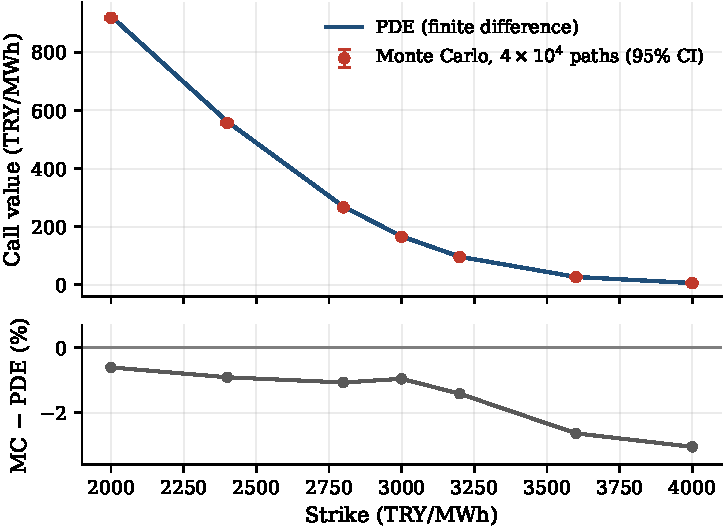
\includegraphics[width=\textwidth]{figures/pde_mc.pdf}
\caption{Finite-difference against Monte Carlo call values at $72$ hours, with
the relative difference below.}
\label{fig:pdemc}
\end{figure}

Agreement of this kind is informative about implementation correctness. It says
nothing about whether the parameters describe the market.

\subsection{The risk-neutral drift channel}
\label{sec:q1}

The regime and volatility parameters of Section~\ref{sec:residual} are
historical estimates under $\PP$. Using them unchanged for valuation asserts
that the market prices neither regime nor volatility risk. Since the monthly
strip cannot identify either premium, we do not attempt to estimate them.
Instead we implement the change of measure explicitly so that the assumption
becomes visible and its consequences measurable.

Following the structure in \citet{Janczura2014}, we admit a regime-dependent
drift perturbation, replacing \eqref{eq:ou} by
\begin{equation}
  \dif X_t = \left[\kappa\left(m_{S_t}-X_t\right) + a_{S_t}\right]\dif t
             + \sigma^X_{S_t}(t)\,\dif W^{\Q}_t,
  \label{eq:q1}
\end{equation}
with $a=(a_0,a_1)$ expressed in \TRY{} per hour. Setting $a=(0,0)$ recovers the
physical-measure baseline exactly, bit for bit, so every result in this paper
that does not explicitly vary $a$ is a zero-premium result and is labelled as
such.

The perturbation enters \eqref{eq:momentsys} through $a_ip_i$ in the first moment
and $2a_iu_i$ in the second, so the effect on the variance, and hence on option
value, is second order in $a$. Appendix~\ref{app:moments} derives the order and
reports the numerical check, a log-log slope of $2.0000$ across
$a_1\in\{-0.5,\dots,-20\}$. At magnitudes plausible for a drift premium the
resulting price change falls below the solver's resolution. The implication is
specific: within this specification a \emph{drift}-type premium is nearly
unidentifiable from option values even if one were observed, because its channel
is quadratically suppressed. A premium shifting transition intensities rather
than drift would not be suppressed in the same way, and that extension is left
open.

\section{Parameter provenance}
\label{sec:provenance}

A valuation model is only as interpretable as the audit trail behind its
inputs. We therefore classify every parameter into one of four categories and
report the classification alongside the value itself.

\begin{description}
\item[Calibrated] determined by observed market prices through the constrained
  optimisation of Section~\ref{sec:curve}.
\item[Inherited] taken from a historical estimation exercise under $\PP$ and
  used for valuation without a measure adjustment.
\item[Derived] reconstructed from summary statistics of that exercise because
  the primary estimate was unavailable, with no standard error attached.
\item[Assumed] chosen by the analyst on economic or pragmatic grounds.
\end{description}

Table~\ref{tab:provenance} applies the scheme. Only the forward curve is
calibrated. Everything governing the distribution around it is inherited,
derived or assumed, which is the concrete form the incompleteness of this
market takes.

\begin{table}[htbp]
\centering
\caption{Production parameters and provenance. Only $F(\cdot)$ is identified by
market prices.}
\label{tab:provenance}
\small
\setlength{\tabcolsep}{4pt}
\begin{tabular}{@{}llll@{}}
\toprule
Parameter & Value & Status & Note \\
\midrule
$F(\cdot)$ & curve & Calibrated & Exact on six monthly averages \\
Jan.\ anchor & \texttt{spot\_to\_next} & Assumed & No quote exists \\
$\kappa$ (h$^{-1}$) & $0.078394$ & Inherited & Half-life $8.84$\,h \\
$\sigma^{y}_{0}$ & $0.0035348$ & Inherited & Calm regime \\
$\sigma^{y}_{1}$ & $0.0924067$ & Inherited & Stress regime \\
$s_P$ (\TRY) & $282.48$ & Assumed & Source file unavailable \\
$\alpha_{01}$ & $-1.015666$ & Derived & Duration reconstruction \\
$\alpha_{10}$ & $-1.895229$ & Derived & Duration reconstruction \\
$\gamma_{01}$ & $-0.583778$ & Inherited & Ramp term omitted \\
$\gamma_{10}$ & $+0.077698$ & Inherited & Ramp term omitted \\
$\pi_{1,0}$ & $0.068023$ & Inherited & Filtered at valuation \\
$a_0,a_1$ & $0,\ 0$ & Assumed & Zero drift premium \\
$r$ (annual) & $0.40$ & Assumed & Flat, not calibrated \\
\bottomrule
\end{tabular}
\end{table}

Three entries require comment because they carry more interpretive weight than
their appearance in a table suggests.

The intercepts $\alpha_{01},\alpha_{10}$ were not available from the original
estimation output, which reported slope coefficients and average marginal
effects but not intercepts. We reconstructed them by solving, over the full
covariate sample, the two scalar equations that match the implied average
departure rates to the reported mean regime durations of $3.76$ and $7.56$
hours. The reconstruction reproduces the reported stationary stress share to
within $1\%$ under an ergodic approximation and $4.5\%$ under simulation along
the realised covariate path. It is nevertheless a moment-matching
reconstruction and not a likelihood estimate, so no standard error attaches to
it and no inference should be drawn from its magnitude.

The slopes $\gamma_{01},\gamma_{10}$ come from a specification that also
contained a residual-demand ramp covariate, which the production implementation
does not carry. If the original fit was joint, our slopes are subject to omitted
variable bias of unknown sign. We were unable to determine from the available
artefacts whether the two covariates were estimated jointly or separately, and
we report the ambiguity rather than resolving it by assumption.

The initial regime distribution $\pi$ comes from a filter run under an earlier
model specification than the one supplying the volatilities, so the production
configuration mixes sources at the initialisation step. We quantify the
consequence directly in Section~\ref{sec:sensitivity} by re-pricing under the
alternative of initialising at the stationary distribution.

\section{Results}
\label{sec:results}

\subsection{Curve reproduction and shape}
\label{sec:curvefit}

The constrained solve reproduces all six monthly averages to a maximum absolute
error of $3.6\times10^{-12}$ \TRY{} (Figure~\ref{fig:monthlyfit}), which
establishes only that the constraint set is satisfied, for the reason given in
Section~\ref{sec:curve}.

\begin{figure}[htbp]
\centering
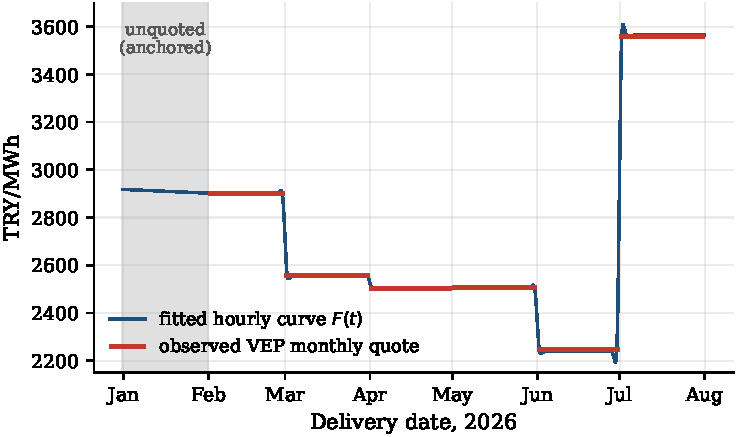
\includegraphics[width=\textwidth]{figures/fwd_curve.pdf}
\caption{Fitted hourly forward curve against the observed monthly baseload
quotes. Shading marks the unquoted January window.}
\label{fig:monthlyfit}
\end{figure}

The shape of the curve is more informative than the fit. Hourly increments have
a mean absolute size of $0.45$ \TRY, and the three largest increments over the
whole horizon sit at month boundaries where the quote strip itself steps, the
largest being $+47.0$ \TRY{} at June--July. That step reflects the $58\%$ rise
between the June and July quotes and is therefore a property of the data rather
than an artefact of interpolation. Within the January window the largest
increment is $0.05$ \TRY, so the anchor joins the quoted region without a
discontinuity, and no oscillation of the kind unconstrained spline interpolation
can produce near sharp level changes is present.

\subsection{Baseline valuation and the option surface}
\label{sec:surface}

At the reference contract, a European call struck at $3{,}000$ \TRY{} expiring
$72$ hours after valuation, the model gives $F(T) = 2{,}916.16$ \TRY, terminal
residual standard deviation $532.26$ \TRY, and a value of $166.75$ \TRY{} by
finite differences against $169.18$ \TRY{} by simulation. The simulated
probability of a negative terminal price is zero at four decimal places, so the
additive specification, while unbounded below in principle, is not operating
near that boundary at the calibrated dispersion.

Table~\ref{tab:surface} reports the surface at three representative strikes,
and Figure~\ref{fig:surface} displays the grid as strike and maturity sections.
Sections are preferred to a perspective surface because exact values remain
readable.

\begin{table}[htbp]
\centering
\caption{Expiry-hour European option values from the production configuration.
All expiries fall inside the unquoted January window. All quantities in \TRY.}
\label{tab:surface}
\small
\begin{tabular}{rrrrrr}
\toprule
Maturity (h) & Strike & $F(T)$ & Call & Put & Residual SD \\
\midrule
\multirow{3}{*}{24}  & 2{,}000 & 2{,}917.24 & 927.11 & 10.87 & \multirow{3}{*}{524.08} \\
                     & 3{,}000 & 2{,}917.24 & 163.93 & 246.60 & \\
                     & 4{,}000 & 2{,}917.24 & 5.59 & 1{,}087.16 & \\
\midrule
\multirow{3}{*}{72}  & 2{,}000 & 2{,}916.16 & 924.70 & 11.55 & \multirow{3}{*}{532.26} \\
                     & 3{,}000 & 2{,}916.16 & 166.75 & 250.32 & \\
                     & 4{,}000 & 2{,}916.16 & 5.94 & 1{,}086.22 & \\
\midrule
\multirow{3}{*}{336} & 2{,}000 & 2{,}910.21 & 907.92 & 11.57 & \multirow{3}{*}{531.19} \\
                     & 3{,}000 & 2{,}910.21 & 161.84 & 250.27 & \\
                     & 4{,}000 & 2{,}910.21 & 5.66 & 1{,}078.86 & \\
\midrule
\multirow{3}{*}{720} & 2{,}000 & 2{,}901.51 & 883.95 & 11.60 & \multirow{3}{*}{529.61} \\
                     & 3{,}000 & 2{,}901.51 & 154.91 & 250.21 & \\
                     & 4{,}000 & 2{,}901.51 & 5.28 & 1{,}068.24 & \\
\bottomrule
\end{tabular}
\end{table}

\begin{figure}[htbp]
\centering
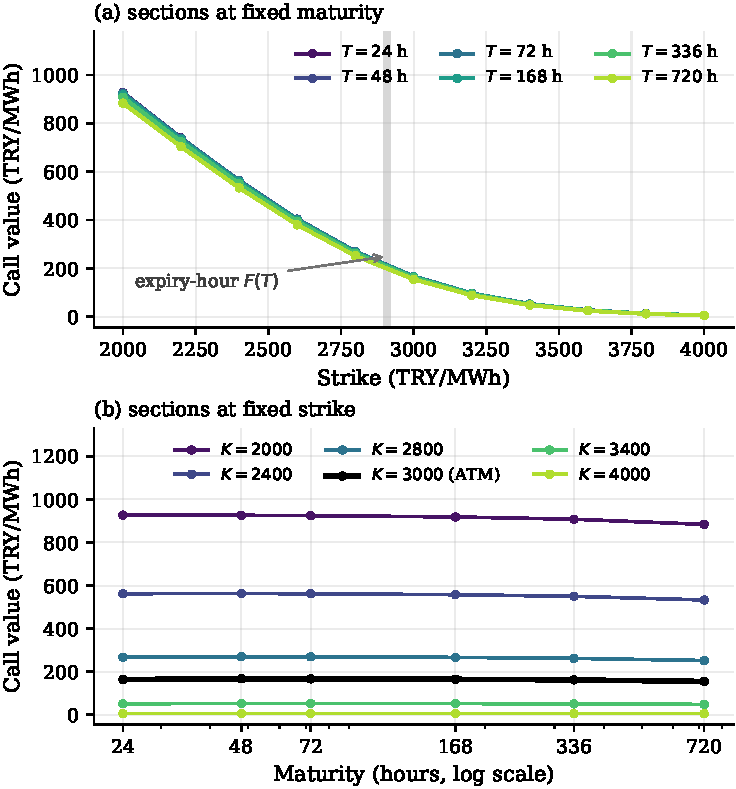
\includegraphics[width=\textwidth]{figures/option_surface.pdf}
\caption{Two sections through the option price surface. Panel (a) shows call
value against strike at each maturity, with shading marking the range of
expiry-hour forward levels; panel (b) shows call value against maturity at
representative strikes, the near-at-the-money strike emphasised.}
\label{fig:surface}
\end{figure}



One feature of the surface separates it from the term structure of a diffusive
model and follows directly from the mean-reverting residual: terminal dispersion
saturates rather than growing (Figure~\ref{fig:residualsd}). With a half-life of
$8.84$ hours the residual reaches its stationary distribution within roughly a
day, after which option value varies with maturity almost entirely through the
forward level and the discount factor rather than through accumulated
uncertainty. The mild decline in at-the-money value across the maturities in
Table~\ref{tab:surface} is therefore attributable to the downward slope of the
anchored January curve rather than to any reduction in volatility.

\begin{figure}[htbp]
\centering
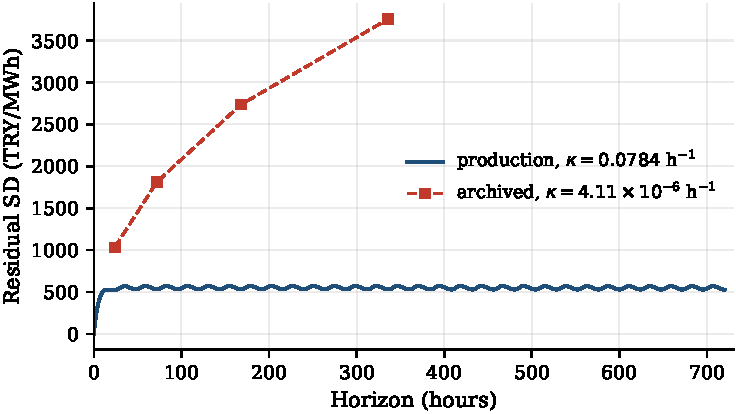
\includegraphics[width=\textwidth]{figures/residual_sd.pdf}
\caption{Terminal residual standard deviation against horizon, production
against archived specification.}
\label{fig:residualsd}
\end{figure}

\subsection{Sensitivity to unidentified inputs}
\label{sec:sensitivity}

Table~\ref{tab:sensitivity} collects controlled experiments in which a single
input is varied and everything else is held at production values. We order them
by the magnitude of the resulting price change, because that ordering is itself
the main result of this section.

\begin{table}[htbp]
\centering
\caption{Controlled sensitivity of the $72$-hour, $K=3{,}000$ call. Each row
varies one input; all others are held at production values. Baseline
$166.75$ \TRY.}
\label{tab:sensitivity}
\small
\setlength{\tabcolsep}{5pt}
\begin{tabular}{@{}llrr@{}}
\toprule
Input varied & Perturbation & Call (\TRY) & Change \\
\midrule
January anchor level & $-20\%$ & 17.80 & $-89.3\%$ \\
January anchor level & $-10\%$ & 65.75 & $-60.6\%$ \\
January anchor level & $+10\%$ & 326.05 & $+95.5\%$ \\
January anchor level & $+20\%$ & 528.96 & $+217.2\%$ \\
\midrule
Mean-reversion rate & archived near-unit-root value & 687.04 & $+312.0\%$ \\
\midrule
Residual demand path & $-2\sigma$ offset & 200.81 & $+20.4\%$ \\
Residual demand path & $+2\sigma$ offset & 107.97 & $-35.2\%$ \\
\midrule
Regime volatilities & alternative model estimate & 165.58 & $-0.70\%$ \\
Discount rate & $r=0.15$ & 167.09 & $+0.21\%$ \\
Discount rate & $r=0.60$ & 166.47 & $-0.16\%$ \\
Initial regime distribution & stationary rather than filtered & 166.75 & $+0.0003\%$ \\
Drift premium $a_1$ & plausible magnitudes & 166.75 & $<10^{-4}\%$ \\
\bottomrule
\end{tabular}
\end{table}

\paragraph{The anchor dominates everything else.}
\label{sec:anchorsens}
Shifting the January anchor level by $\pm20\%$, holding the curve shape rule
fixed, moves the call by $-89\%$ to $+217\%$ (Figure~\ref{fig:anchorsens}); no
other input comes within an order of magnitude. The mechanism is simple. The
anchor sets the forward level at expiry, moneyness dominates the value of a
near-at-the-money option, and the residual dispersion of roughly $530$ \TRY{} is
small against a $\pm580$ \TRY{} shift in the forward. The practical implication
is direct: where the nearest delivery month is unquoted, the precision of any
reported option value is bounded above by the uncertainty in the near-term
forward level, and refinements to the residual specification cannot improve on
that bound. A single reported price is then less informative than the
anchor-conditional range.

\begin{figure}[htbp]
\centering
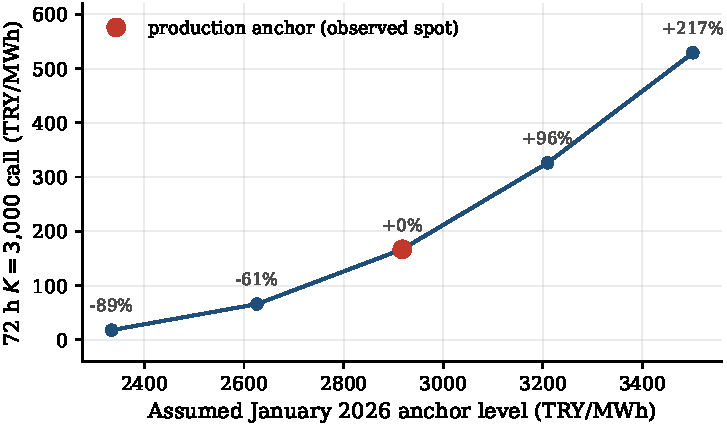
\includegraphics[width=\textwidth]{figures/anchor_sensitivity.pdf}
\caption{Option value against the assumed January anchor level, curve shape
rule held fixed.}
\label{fig:anchorsens}
\end{figure}

\paragraph{Persistence is the dominant residual-layer input.}
The archived specification inherited its mean-reversion rate from an
autoregressive fit to the untransformed price level, giving
$\phi = 0.999996$, $\kappa = 4.11\times10^{-6}$ h$^{-1}$ and a within-regime
half-life near nineteen years. Under that value the same contract prices at
$687.04$ \TRY, more than four times the production figure, because a
near-unit-root residual accumulates variance almost linearly in horizon instead
of saturating. The correction substitutes the deseasonalised single-regime
coefficient $\phi = 0.9246$, giving $\kappa = 0.0784$ h$^{-1}$ and the
saturating dispersion path of Figure~\ref{fig:residualsd}.

The two figures are not in conflict once the objects are separated. A
Markov-switching AR(1) has a marginal autocorrelation that mixes a fast
component, decaying at rate $q_{01}+q_{10}\approx 0.398$ h$^{-1}$, with a slow
component decaying at $-\ln\phi$. Because the regime-conditional means here are
small and close together, the regime-shift contribution to variance is around
$5\%$, so the marginal autocorrelation is dominated by the slow component. A
$200{,}000$-hour simulation confirms an empirical half-life consistent with the
near-unit-root value to within $2\%$ of theory. The nineteen-year figure
correctly describes persistence of the raw transformed price, which over the
estimation window absorbs lira depreciation; it does not describe persistence of
deviations around a forward curve, which is the object \eqref{eq:ou} requires.
Diagnosing this took separating two quantities that a single reported statistic
had conflated.

\paragraph{What the centring buys.}
Running the same parameter set through the archived multiplicative specification
of Remark~\ref{rem:multiplicative}, which lets the residual dynamics determine
the implied forward rather than anchoring it, gives Figure~\ref{fig:legacy}. The
centred form returns $F(T)$ at every horizon. The multiplicative form, on
identical parameters, converges instead to an implied expected spot near
$-3{,}108$ \TRY{} against an observed forward of $+2{,}916$ \TRY. The sign
arises from the regime-weighted mean in transform space rather than from the
variance inflation dominating under the archived mean-reversion rate, so the
specification fails differently at different parameter values while failing in
both. This is the practical content of Proposition~\ref{prop:centering}: forward
consistency is either imposed or it is not obtained.

\begin{figure}[htbp]
\centering
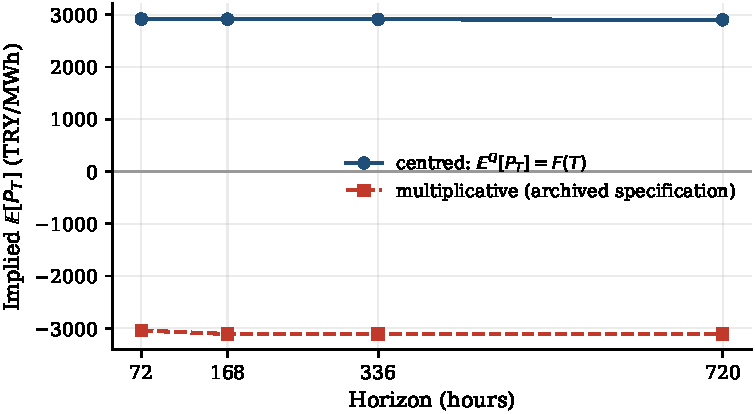
\includegraphics[width=\textwidth]{figures/legacy_vs_centered.pdf}
\caption{Implied expected spot, centred against archived multiplicative
specification.}
\label{fig:legacy}
\end{figure}

\paragraph{The covariate channel is economically signed.}
Shifting the residual demand path by $-2\sigma$ raises the call by $20.4\%$ and
by $+2\sigma$ lowers it by $35.2\%$ (Figure~\ref{fig:rdsweep}), with terminal
dispersion moving from $608$ to $404$ \TRY{} across the same range. The sign
follows from the estimated slopes: $\gamma_{01}<0$ means high residual demand
suppresses transitions into the high-variance regime in this specification.

That direction runs against the intuition that scarcity drives volatility, and
it deserves comment. Two considerations make it less surprising than it first
appears. The regimes here are variance states in transform space rather than
economic stress states, as Appendix~\ref{app:transitions} notes, so the relevant
question is when hourly price variability is large rather than when prices are
high. And low residual demand is precisely the condition under which
renewable output displaces the flexible thermal units that would otherwise
absorb short-run imbalances, leaving a supply stack with less capacity to
respond smoothly. The realised sample is consistent with this reading: across
the seven evaluation months, the correlation between the monthly mean price and
the monthly standard deviation of realised prices is $-0.67$, with the
highest-price month showing the lowest dispersion ($573$ \TRY) and one of the
lowest-price months the highest ($1{,}258$ \TRY). With seven observations this
is suggestive rather than conclusive, and we do not treat it as a test.

The direction is therefore reported as a property of the estimated coefficients,
not as an established economic finding, since the omitted ramp covariate
documented in Section~\ref{sec:provenance} could alter it and the intercepts
entering the same logistic functions are reconstructions rather than estimates.

\begin{figure}[htbp]
\centering
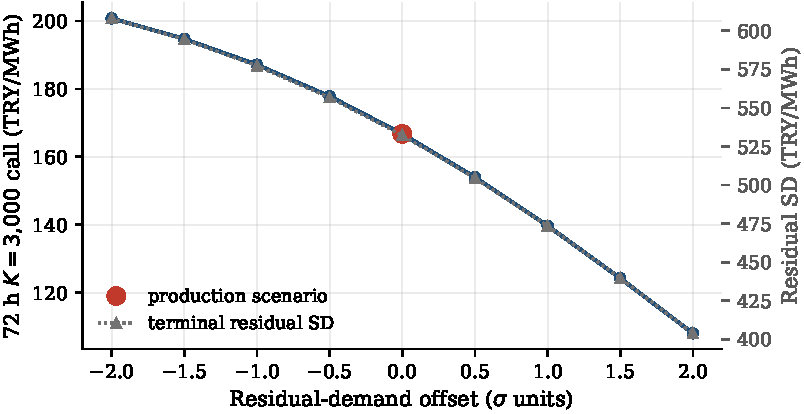
\includegraphics[width=\textwidth]{figures/rd_sweep.pdf}
\caption{Call value and terminal dispersion across a $\pm2\sigma$ range of
residual-demand offsets.}
\label{fig:rdsweep}
\end{figure}

\paragraph{Everything else is second order.}
Substituting the regime volatilities of the closest competing estimated model
changes the price by $0.70\%$, despite a large difference in fit criteria between
the two specifications. The discount rate is similarly immaterial across
$r\in[0.15,0.60]$, a range bracketing Turkish policy rates over the period: at
$720$ hours the factor $e^{-rT}$ moves only from $0.988$ to $0.952$. That is a
property of the maturities studied rather than evidence that the assumption is
innocuous in general, and contracts extending over several months would require
the term structure of rates to be modelled rather than assumed. Initialising the
chain at its stationary distribution rather than the filtered one is likewise
immaterial at $72$ hours, since with mean regime durations under eight hours the
chain has forgotten its initial condition well before expiry; the same
substitution moves a $6$-hour option by roughly $29\%$, so the irrelevance again
belongs to the horizon rather than to the parameter. The drift premium channel is
quadratically suppressed, as established in Section~\ref{sec:q1}.

\subsection{Realised evaluation}
\label{sec:realised}

The forward curve constructed at the end of 2025 can be compared against what
subsequently occurred. Table~\ref{tab:realised} reports, for each delivery month,
the realised mean, the bias of the curve against it, the mean absolute error, the
symmetric percentage error, and a dispersion ratio comparing mean model residual
standard deviation to the realised standard deviation of realised-minus-forward
within that month. Figure~\ref{fig:backtest} plots the two series as daily means together with the
monthly biases, the January bar distinguished because its level comes from the
anchor rather than from a quote.

\begin{table}[htbp]
\centering
\caption{Realised evaluation against the production forward curve, January to
July 2026.}
\label{tab:realised}
\small
\setlength{\tabcolsep}{4.5pt}
\begin{tabular}{@{}lrrrrrr@{}}
\toprule
Month & Hours & Realised mean & Bias & MAE & sMAPE & Disp.\ ratio \\
\midrule
2026-01$^{\dagger}$ & 744 & 2{,}894.92 & $-14.47$ & 451.93 & 16.8\% & 0.97 \\
2026-02 & 672 & 2{,}078.20 & $-822.79$ & 992.40 & 50.0\% & 0.56 \\
2026-03 & 744 & 1{,}620.32 & $-935.99$ & 1{,}193.58 & 71.5\% & 0.46 \\
2026-04 & 720 & 921.06 & $-1{,}579.60$ & 1{,}873.41 & 126.3\% & 0.41 \\
2026-05 & 744 & 590.90 & $-1{,}915.35$ & 2{,}150.69 & 155.2\% & 0.44 \\
2026-06 & 720 & 1{,}240.16 & $-1{,}005.17$ & 1{,}458.19 & 101.3\% & 0.35 \\
2026-07 & 744 & 2{,}699.61 & $-858.58$ & 1{,}058.33 & 40.9\% & 0.61 \\
\midrule
Overall & 5{,}088 & 1{,}721.72 & $-1{,}019$ & 1{,}312.39 & 80.4\% & --- \\
\bottomrule
\end{tabular}

\vspace{2pt}
\footnotesize $^{\dagger}$ January carries no observed quote; its curve level
is the near-term anchor assumption.
\end{table}

\begin{figure}[htbp]
\centering
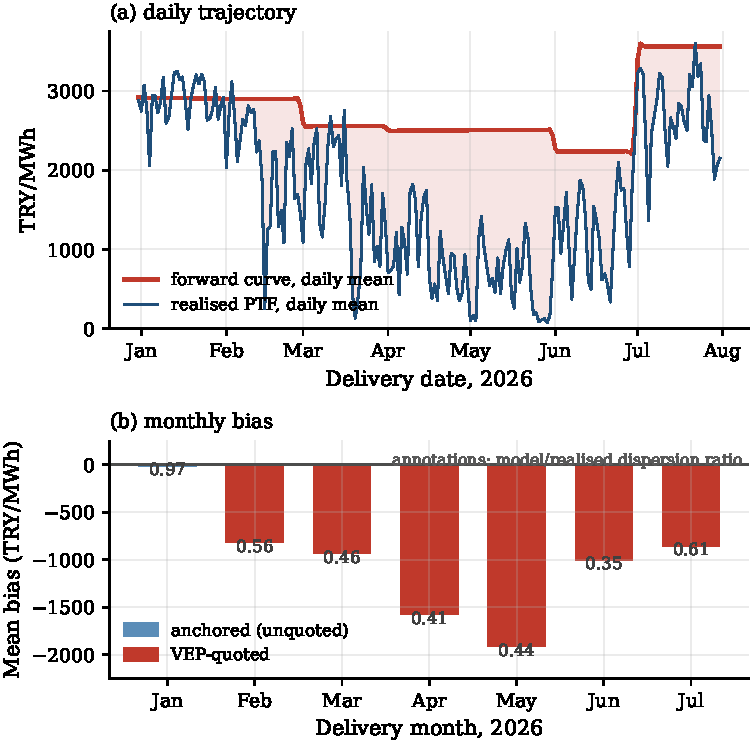
\includegraphics[width=\textwidth]{figures/backtest.pdf}
\caption{Realised evaluation. Panel (a) plots realised PTF against the
production forward curve as daily means; panel (b) gives the monthly mean bias,
with the anchored January window distinguished from the VEP-quoted months.}
\label{fig:backtest}
\end{figure}



Three observations follow, and we state them in order of how much they
constrain the interpretation of the rest of the paper.

First, the forward strip missed badly. Realised prices fell below the quoted
forward in every month from February onwards, by $24\%$ in July and by $76\%$ in
May, with an overall mean bias of $-1{,}019$ \TRY. In May, $222$ of $744$
delivery hours cleared below $10$ \TRY. The magnitude of the deviation is
consistent with a large supply-side shock rather than with ordinary forecast
error, and the period coincided with exceptionally favourable hydrological
conditions and record renewable output that displaced gas-fired generation from
the merit order. We describe the coincidence and do not estimate it; attributing
the deviation causally would require a supply-stack decomposition that we do not
perform, and the merit-order mechanism is well documented elsewhere
\citep{Sensfuss2008,Ketterer2014,Clo2015,SirinYilmaz2020}.

Second, because our curve reproduces the quotes exactly, the entire level error
is inherited from the forward market. No property of the residual
specification, the regime structure or the pricing scheme contributed to it. The
error therefore bounds what forward-anchored valuation can deliver in this
market, and the bound is not a small one: an option value anchored to a forward
curve that is subsequently wrong by $40\%$ on average is wrong by a
correspondingly large amount, however carefully the distribution around the
curve was specified. This is a structural property of the anchoring approach
rather than a defect of our implementation, and it applies equally to any of the
curve-construction methods cited in Section~\ref{sec:curve}.

Third, the month that was not quoted performed best. January, whose level came
entirely from the near-term anchor assumption, shows a bias of $-14.47$ \TRY{}
and the lowest sMAPE in the sample, while every quoted month missed by hundreds
of lira. We caution against reading this as evidence that the anchor rule
outperforms the market. The anchor was set at the observed spot and interpolated
towards February, so it inherited the information content of a price observed
one hour before the window opened, whereas the quoted months encode expectations
formed up to seven months ahead. The comparison illustrates how rapidly forward
information decayed during this episode rather than the merits of an
interpolation rule.

\subsection{Evidence from seven valuation dates}
\label{sec:multidate}

A single valuation date cannot distinguish an unusual episode from a persistent
property of the quote strip. The curve construction can be replayed at earlier
dates without contamination, because it uses only the quotations published on
the valuation date and the spot of that hour and contains no historical
parameter. The residual dynamics cannot be replayed, since their parameters are
fitted to data through 2025, so this exercise evaluates the forward curve alone
and prices no option. Seven valuation dates at six-month intervals from
2022-12-31 to 2025-12-31 yield $49$ (date $\times$ delivery month)
observations. Replaying 2025-12-31 through the same code reproduces the
published curve to $4.5\times10^{-13}$ \TRY{} over $5{,}089$ hours.

Three results follow, and the first revises the reading of
Section~\ref{sec:realised}.

\paragraph{The front month is never quoted.} The anchor rule fires at all seven
dates. Every strip prices delivery months two through seven ahead and none
prices the first, so the structural claim of Section~\ref{sec:anchor} holds
across three years rather than resting on one observation.

\paragraph{2026 is large but not exceptional.} The $-1{,}019$ \TRY{} mean bias
of the 2025-12-31 curve sits at the $32.7$th percentile of the pooled
distribution and the $28.6$th percentile of the seven date means, inside their
interquartile range. Two earlier dates produced more negative outcomes, the
worst being 2022-12-31 at $-1{,}465$ \TRY{} ($-39.8\%$). The hydrological
episode of 2026 is therefore an instance of a magnitude the strip has produced
before, not a departure from otherwise reliable behaviour.

\paragraph{The bias is large, negative on average, and unstable in sign.}
Pooled across dates the mean bias is $-603$ \TRY{} ($-18.2\%$ in relative terms)
with a standard deviation of $775$ \TRY. Realised prices came in below the strip
at five dates and above it at two, with date means running from $-1{,}465$ to
$+290$ \TRY{} (Figure~\ref{fig:multidate}a). The direction is not a stable
property. Statistical support for a non-zero mean is correspondingly weak once
dependence is respected: pooling all $49$ observations gives $t=-5.45$, but the
same delivery month appears from several valuation dates and consecutive months
of one curve share a market state, so that figure is anti-conservative.
Aggregating to one observation per date gives $t=-2.29$ on seven dates,
$p=0.062$, and restricting to non-overlapping delivery windows leaves $p$
between $0.11$ and $0.49$. We therefore report the mean bias as economically
large and describe the strip as a biased and unstable predictor, without
claiming a calibrated significance level on seven dates.

\begin{table}[htbp]
\centering
\caption{Mean bias of the forward curve against realised monthly baseload, by
valuation date. Seven delivery months per date.}
\label{tab:multidate}
\small
\setlength{\tabcolsep}{6pt}
\begin{tabular}{@{}lrrr@{}}
\toprule
Valuation date & Mean bias (\TRY) & Median (\TRY) & Relative (\%) \\
\midrule
2022-12-31 & $-1{,}464.63$ & $-1{,}545.59$ & $-39.8$ \\
2023-06-30 & $-1{,}250.01$ & $-1{,}299.88$ & $-36.5$ \\
2023-12-31 & $-756.89$    & $-813.27$     & $-24.5$ \\
2024-06-30 & $-174.47$    & $-214.48$     & $-6.2$ \\
2024-12-31 & $+151.28$    & $+179.60$     & $+7.2$ \\
2025-06-30 & $+289.76$    & $+307.18$     & $+11.4$ \\
2025-12-31 & $-1{,}018.85$ & $-935.99$    & $-39.1$ \\
\midrule
Pooled ($n=49$) & $-603.40$ & $-353.70$ & $-18.2$ \\
\bottomrule
\end{tabular}
\end{table}

\begin{figure}[htbp]
\centering
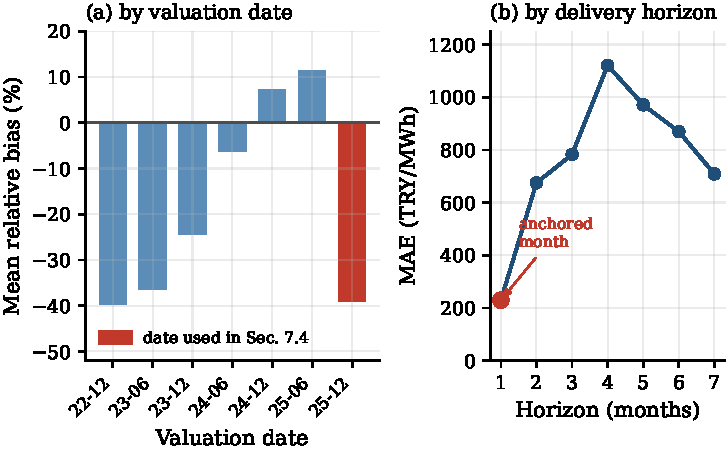
\includegraphics[width=\textwidth]{figures/multi_date.pdf}
\caption{Forward curve error across seven valuation dates. Panel (a) gives the
mean relative bias per date; panel (b) the mean absolute error by delivery
horizon.}
\label{fig:multidate}
\end{figure}

\paragraph{The anchor band has approximately the right scale.} The $\pm20\%$
band used in Section~\ref{sec:anchorsens} was chosen without empirical support.
Across the seven anchored months the realised relative error has a standard
deviation of $11.7\%$, against $11.5\%$ for a uniform distribution on
$\pm20\%$, so the band is of the right width. It is not a containment bound:
one of seven anchored months falls outside it, at $-21.2\%$. And its centre is
displaced, the empirical mean being $-3.5\%$, so the linear ramp over-prices the
anchored month slightly on average. The band should be read as a scale for
anchor uncertainty rather than as a range that brackets it.

\paragraph{Error does not grow monotonically with horizon.}
Figure~\ref{fig:multidate}b shows mean absolute error rising from $229$ \TRY{}
at the anchored first month to $1{,}121$ \TRY{} four months ahead, then falling
back to $708$ \TRY{} at seven, with a Spearman rank correlation of $+0.25$
between horizon and absolute error. The decline at the long end should not be
read as skill. The first horizon is always the anchored month, so its small
error reflects a ramp from an observed spot rather than a quoted forward, and
with dates six months apart the seventh horizon is always the same pair of
calendar months, making the long end as much seasonal as maturity-driven.

Four of the seven valuation dates fall on a non-business day, when no index
price is published; for those the strip is the last publication before the date,
one to four days stale, while the spot remains that of the valuation night. No
later publication is used anywhere, the affected observations are flagged in the
released data rather than dropped, and a strict same-day rule would reduce the
study to three dates.

A fourth observation concerns the model's own dispersion. The ratio of model
residual standard deviation to realised dispersion is $0.97$ in January and
falls to $0.35$--$0.61$ thereafter, so outside the anchored window the model is
too narrow by a factor of roughly two. Part of this is expected: the production
residual is a single-factor approximation, and a companion two-factor
specification developed alongside this work carries an additional slow component
that the production configuration does not represent. Part is the shock itself,
which widened realised dispersion beyond anything the historical sample
contains. We do not attempt to separate the two here.

\section{Discussion}
\label{sec:discussion}

\subsection{What a monthly strip identifies}

The results support a narrow reading of what calibration to a baseload strip
accomplishes. It fixes six linear functionals of a curve with several thousand
degrees of freedom, and through Proposition~\ref{prop:centering} it fixes the
first moment of the price distribution at every horizon. It does not fix the
intraday shape of the curve, the level over unquoted months, the volatility of
deviations around the curve, or any risk premium. The sensitivity ordering in
Table~\ref{tab:sensitivity} makes the consequence concrete: the largest single
driver of the reported option value is an input that no observed price
constrains.

A reporting convention follows. Rather than a point value, valuation in markets
of this type is better expressed as a value conditional on an explicitly stated
anchor, accompanied by the range induced by plausible alternatives. The $\pm20\%$
anchor band used here produces a call range of $17.80$ to $528.96$ \TRY{} around
a central $166.75$ \TRY, and that interval carries more information than its
midpoint. Section~\ref{sec:multidate} supplies the band with a warrant it
previously lacked: across seven valuation dates the realised anchor error has a
standard deviation of $11.7\%$, close to the $11.5\%$ a uniform $\pm20\%$ prior
implies, though displaced by $-3.5\%$ from zero and not containing the tail.

\subsection{What the strip predicts, and what that costs}

The multi-date evidence bears on a question wider than valuation mechanics.
Whether forward prices are unbiased predictors of subsequent spot outcomes is an
old subject in electricity markets, where limited storage and inelastic demand
make the hedging-pressure equilibrium of \citet{BessembinderLemmon2002} a natural
frame and where realised premia have been measured for mature markets by
\citet{LongstaffWang2004} and \citet{Algieri2021}. On Turkish monthly baseload
contracts over 2023--2026, the answer is that the strip is neither unbiased nor
reliably biased in one direction. Its pooled error averages $-18\%$ of the
forward level, so a buyer of the strip paid on average well above what delivery
subsequently cost; but two of seven dates reversed the sign, and the date-level
mean is not distinguishable from zero at conventional levels once the dependence
between overlapping windows is respected.

For anyone using such a curve, the practical consequence is about capital rather
than about point forecasts. A dispersion of $775$ \TRY{} around a mean of
$-603$ \TRY{} on a price level near $2{,}500$ \TRY{} means the position risk of a
forward-anchored book is dominated by the level of the curve it is anchored to,
not by the shape of the distribution placed around that level. Provisioning
against the residual volatility of Section~\ref{sec:results}, terminal dispersion
of roughly $530$ \TRY{} at the horizons studied, while treating the anchor level
as known would understate the exposure by a wide margin. The ordering in
Table~\ref{tab:sensitivity} says the same thing from the pricing side, and the
multi-date distribution is what puts a number on it.

We stop short of decomposing the error into a risk premium and a forecast error.
Separating the two requires either an instrument for expectations or a structural
model of the supply stack, and seven valuation dates would not identify it. That
the strip was systematically above realised outcomes in the years when hydrology
was favourable, and below in the years when it was not, is consistent with both a
premium and a persistent forecasting difficulty, and this sample cannot
distinguish them.

\subsection{Separation of concerns as a design property}

The centring identity does more than tidy the algebra. It creates a firewall
between the market-identified and the assumed parts of the model, and the value
of that firewall emerged in a way that had not been anticipated when it was
adopted. When the inherited mean-reversion rate was found to be wrong by four
orders of magnitude, the correction changed option values by a factor of four
while leaving the forward reproduction, the monthly fit errors and the realised
level bias unchanged. In a specification where residual dynamics fed back into
the implied forward, everything would have required recalibration and the
diagnosis would have been considerably harder, since the symptom would have
surfaced in the calibration layer rather than only in the dispersion.

The same property holds for the measure change. Because the drift perturbation
enters both the moment system and the pricing equation through a shared field,
$\E^{\Q}[P_t] = F(t)$ survives any $(a_0,a_1)$, verified numerically at
magnitudes far outside any economically plausible range. Risk premium
assumptions can therefore be explored without disturbing the calibration, which
is what makes them reportable as sensitivities rather than as a separate model.

\subsection{Persistence, transformation and nominal prices}

The mean-reversion episode carries a methodological lesson that generalises
beyond this dataset. Reported persistence statistics from a regime-switching
estimation describe several distinct objects: within-regime autoregressive
persistence, the marginal persistence of the observed series, and the persistence
of deviations around a reference curve. These coincide only under restrictive
conditions. Where the estimation sample also spans substantial currency
depreciation, the raw series carries a monetary trend that inflates measured
persistence further, and a coefficient transferred from that context into a
residual-dynamics role will overstate memory by whatever the trend contributes.
Diagnosis here required reconstructing the marginal autocorrelation of the
switching process analytically and verifying it by simulation, since neither
reported statistic alone identified the problem.

This is likely a common failure mode wherever parameters are handed between
modelling stages, and particularly so in emerging markets where nominal series
are non-stationary for reasons unrelated to the physics of the power system. The
defence that eventually worked is worth stating as a rule: every transferred
parameter should name the process it was estimated on, and any mismatch between
that process and its intended use should be treated as an error until shown
otherwise.

\section{Limitations and future work}
\label{sec:limitations}

\paragraph{Identification.} Volatility and regime risk premia are not identified
by a monthly baseload strip, and no attempt is made here to estimate them. All
reported values are zero-premium values in the sense of Section~\ref{sec:q1}.
A drift-type premium is additionally quadratically suppressed within this
specification, so even option data might identify it only weakly; an
intensity-type premium is the more promising target and is not implemented.

\paragraph{Parameter provenance.} Three items in Table~\ref{tab:provenance}
carry unresolved questions. The transition intercepts are moment-matching
reconstructions without standard errors. The transition slopes come from a
specification containing a ramp covariate that the production implementation
omits, with omitted-variable consequences of unknown sign. The transform scale
$s_P=282.48$ could not be verified because the preprocessing metadata defining it
was unavailable; it is a median absolute price over a training window spanning
years of substantial lira depreciation, so the price regime it represents may
differ materially from that at the valuation date. Each would be resolved by
access to the original estimation artefacts.

\paragraph{Specification scope.} The production residual is a single-factor
mean-reverting process, unbounded below, whereas realised prices face
administrative floors and ceilings. A companion specification developed alongside
this work adds a slow second factor and explicit price limits. It is not
integrated here because clipping the state distribution breaks the centring
identity of Proposition~\ref{prop:centering}: restoring $\E^{\Q}[P_t]=F(t)$ under
a clipped law requires redesigning the centring term rather than adding a bound
to the existing one. The trade-off is worth stating explicitly, because the
obvious alternative is worse. Multiplicative or log-type specifications respect
the lower bound automatically, but under Jensen's inequality their first moment
depends on the residual variance, so forward consistency can no longer be
imposed algebraically. Figure~\ref{fig:legacy} quantifies what that costs on
this data, and the forward inconsistency it shows is larger by orders of
magnitude, measured in \TRY, than the boundary violations the additive form
permits, whose simulated probability at the calibrated dispersion is zero to
four decimal places. That is the most substantive extension available and is
treated as the natural next study rather than a patch to this one. The dispersion
ratios in Table~\ref{tab:realised} indicate what a second factor would need to
supply. The price limit schedule used by the companion specification was inferred
from realised price behaviour rather than read from a primary regulatory
document, and is marked accordingly; it plays no role in the production results.

\paragraph{Evaluation.} The option-level evaluation still rests on a single
valuation date, because the residual parameters cannot be replayed at earlier
dates without look-ahead bias. Only the forward curve is evaluated across the
seven dates of Section~\ref{sec:multidate}, and the two exercises therefore
answer different questions. Seven dates six months apart also leave the delivery
windows partially overlapping and the long horizons confounded with calendar
month, so the horizon profile in particular should be read as descriptive.
Four of the seven strips were published one to four days before their valuation
date because the date fell on a non-business day; a strict same-day rule would
reduce the sample to three. Extending the panel as further quotations and
outturns accumulate, and re-estimating the residual process at each date so that
option prices could also be evaluated out of sample, are the natural
continuations.

\section{Conclusion}
\label{sec:conclusion}

A valuation framework has been developed for expiry-hour electricity options in a
market that supplies a sparse monthly forward strip and no option prices. Its
organising principle is a separation between what such a market identifies and
what it does not. An equality-constrained hourly curve carries the identified
information, a regime-switching residual with residual-demand-driven transition
probabilities carries the assumed distributional structure, and a centring term
ensures the two meet without the second contaminating the first:
$\E^{\Q}[P_t]=F(t)$ holds for every admissible parameter vector, as an algebraic
identity rather than a calibration target.

Applying the framework to Turkish data yields three findings. The dominant source
of uncertainty in the reported option value is the forward level over the
unquoted nearest delivery month, which overwhelms every parameter of the residual
specification by an order of magnitude. The mean-reversion rate is the dominant
residual-layer input, and transferring it from an autoregression on the
untransformed price level rather than on deviations around the curve inflated
option values by a factor of four until diagnosed. And the forward strip itself is a poor predictor of what follows: across seven
valuation dates the mean error is $-18\%$ of the forward level, negative at five
dates and positive at two, with the much-discussed 2026 outcome lying inside the
interquartile range rather than outside it.

The last of these deserves emphasis. Forward-anchored valuation inherits the
predictive accuracy of the forward market entirely, and on this evidence that
accuracy is low and unstable in sign for reasons no pricing model can correct.
Combined with the finding that the nearest delivery month is never quoted, the
implication for practice is that a single option value in this market conveys
less than the value reported together with the range implied by the inputs no
price identifies. What that discipline looks like in practice is what this paper
has tried to demonstrate, including where it revealed our own errors.


\appendix
\section{Derivation of the moment system}
\label{app:moments}

Let $S$ be the two-state chain with generator $Q(t)$ from \eqref{eq:generator}
and let $X$ solve \eqref{eq:q1}. Write $f_i(x,t)$ for the joint density of
$(X_t,S_t=i)$. The forward equation for the pair is
\begin{equation}
  \partial_t f_i
  = -\partial_x\!\left[\left(\kappa(m_i-x)+a_i\right)f_i\right]
    + \tfrac12\left(\sigma^X_i\right)^2\partial_{xx} f_i
    + q_{ji}f_j - q_{ij}f_i,
  \qquad j\neq i .
\end{equation}
Multiplying by $1$, $x$ and $x^2$ and integrating over $x\in\mathbb{R}$, with
the boundary terms vanishing because $f_i$ and $x f_i$ decay at infinity, gives
the system \eqref{eq:momentsys} in the variables
$p_i=\int f_i\,\dif x$, $u_i=\int x f_i\,\dif x$ and $w_i=\int x^2 f_i\,\dif x$.
The three blocks are recursively coupled: $p$ is autonomous, $u$ depends on
$p$, and $w$ depends on $u$ and $p$. The system is therefore linear and
non-autonomous, with time dependence entering through $q_{ij}(t)$ along the
covariate path and through $\sigma^X_i(t)$ via \eqref{eq:sigmamap}.

\paragraph{Order of the drift perturbation.} Write $u_i = u_i^{(0)} + a\,u_i^{(1)} + O(a^2)$
for a perturbation of size $a$. The $u$ block gains the forcing $a_ip_i$, so
$u^{(1)}$ is $O(1)$ and $u$ is first order in $a$. The $w$ block gains
$2a_iu_i$, a product of two quantities each first order in $a$ after
subtracting the baseline, so the variance response is $O(a^2)$. This is the
analytic counterpart of the log-log slope of $2.0000$ reported in
Section~\ref{sec:q1}.

We record one caveat against over-reading the result. The suppression concerns
the variance channel and hence the leading effect on option value. For a
non-at-the-money contract under a centred conditional-Gaussian perturbation, the
first derivative of the call value with respect to a regime-dependent drift need
not vanish identically, since the perturbation also reweights the regime mixture
entering the terminal payoff. The numerical experiments in
Section~\ref{sec:q1} bound the total effect at plausible magnitudes; they do not
establish a general second-order proposition, and we do not claim one.

\section{Transition reconstruction and label reconciliation}
\label{app:transitions}

\paragraph{Label orientation.} The estimation output orders regimes by the raw
fitted index, in which state $0$ carries the higher diffusion coefficient and
occupies roughly $67\%$ of the sample with a mean duration of $7.56$ hours,
while state $1$ carries the lower coefficient and a mean duration of $3.76$
hours. Our convention is the opposite, with index $0$ denoting the calm regime.
Adopting it requires swapping the volatilities and, because the logistic
coefficients are indexed by the same labels, swapping the transition
coefficients crosswise: the production $\gamma_{01}$, governing calm-to-stress
transitions, is the raw $\gamma_{10}$, and conversely. Failing to apply the
swap to both objects would produce a model in which volatilities and transition
dynamics refer to different states, which is a silent error rather than one that
any single diagnostic would reveal. We enforce the ordering with an invariant
check requiring $\sigma^y_0 < \sigma^y_1$ at load time.

The orientation is worth a remark on its own terms. A high-volatility state that
is both dominant and longer-lived inverts the usual reading in which stress is
rare and brief. Whether this reflects genuine market structure at hourly
frequency, or the labelling of a transform-space variance decomposition that
does not correspond to economic stress, we cannot determine from the available
artefacts, and we use the terms calm and stress throughout as labels for
variance states rather than as economic claims.

\paragraph{Intercept reconstruction.} Slope coefficients and average marginal
effects are supplied by the estimation output, but intercepts are not. The mean
departure rate from state $i$ over the covariate distribution must match the
reported mean duration $d_i$, which gives
\begin{equation}
  \E_z\!\left[\Lambda\!\left(\alpha_{01}+\gamma_{01}z\right)\right]
     = \frac{1}{d_{\text{calm}}},
  \qquad
  \E_z\!\left[\Lambda\!\left(\alpha_{10}+\gamma_{10}z\right)\right]
     = \frac{1}{d_{\text{stress}}},
\end{equation}
for $\alpha_{01}$ and $\alpha_{10}$ separately, taking the expectation over the
full standardised covariate sample and using a monotone bracketing root finder.
The target rates are $0.2660$ and $0.1323$ per hour. The resulting pair
reproduces the reported stationary stress share of $0.6746$ to within $1.0\%$
under an ergodic approximation and $4.5\%$ under simulation along the realised
covariate path.

This is moment matching, not estimation. The reconstructed intercepts have no
sampling distribution, no standard errors and no likelihood interpretation, and
any inference conditioned on their precise values would be unfounded. They are
reported as Derived in Table~\ref{tab:provenance} for that reason.

\section{Numerical implementation and verification}
\label{app:numerics}

\paragraph{Moment integration.} The system \eqref{eq:momentsys} is advanced with
classical fourth-order Runge--Kutta and internal sub-stepping capped at $0.25$
hours, with coefficient paths interpolated linearly within each step. The cap is
necessary rather than conservative: on hourly steps without sub-stepping the
second-moment trajectory exhibited visible instability at the calibrated
switching intensities, which propagated into terminal dispersion.

\paragraph{Spatial discretisation.} The coupled system \eqref{eq:pde} is solved
on a uniform grid of $1{,}201$ nodes in the residual coordinate, with the domain
set wide enough that the terminal density is numerically negligible at the
boundaries. The regime coupling term is treated within the same implicit step as
the diffusion, so the two value functions advance together.

\paragraph{Verification.} Three checks are run as automated regressions rather
than as one-off diagnostics, so that any future change to the code that breaks
them fails visibly.
\begin{enumerate}
\item \emph{Put--call parity}: $\max\lvert C-P-e^{-rT}(F(T)-K)\rvert
      = 1.0\times10^{-6}$ \TRY{} across the $66$-point strike--maturity grid.
\item \emph{Centring identity}: $\max_t\lvert\E^{\Q}[P_t]-F(t)\rvert<10^{-8}$
      \TRY{} under drift perturbations including asymmetric and mixed-sign
      pairs, with a companion assertion that the uncentred residual mean is
      meaningfully non-zero so that the test cannot pass vacuously.
\item \emph{Independent resimulation}: $20{,}000$ Monte Carlo paths at a
      $0.05$-hour step with an exact conditional Ornstein--Uhlenbeck update on
      the sampled regime path, giving $169.18$ \TRY{} against $166.75$ \TRY{}
      from finite differences at the reference contract.
\end{enumerate}

We are explicit about what these checks do and do not establish. Parity and the
centring identity test internal consistency of the implementation. The Monte
Carlo comparison tests that two structurally different numerical routes to the
same expectation agree. None of them provides evidence that the parameters
describe the market, and the realised evaluation of Section~\ref{sec:realised}
is the only exercise in this paper that bears on that question.

\paragraph{Reproducibility.} All tables and figures in this paper are generated
from a versioned snapshot of the code and inputs. The full automated test suite
comprises $207$ tests covering the invariants above, the curve construction, the
parameter loader, provenance detection and the regression baselines reported
here.


\bibliographystyle{elsarticle-harv}
\bibliography{refs}

\end{document}
